\documentclass[12pt]{book}

\title{The dark version\\ \textit{better to burn out than to fade away}
\begin{center}
\includegraphics[width=2in]{org/art/cannabis.png}\end{center}
}

\setlength{\parskip}{.5cm}

%\usepackage[margin=1in]{geometry}

\usepackage{listings}
\lstset{numbers=left,basicstyle=\scriptsize \ttfamily \color{codecolour},language=}

\usepackage{color}
\definecolor{codecolour}{RGB}{180, 180, 180}
\definecolor{tipcolour}{RGB}{50, 50, 50}
\definecolor{pagecolour}{RGB}{180, 180, 180}
\pagecolor{black}
\color{pagecolour}

\usepackage{graphicx}
\usepackage{wrapfig}

\begin{document}
\maketitle

% Where to find things
% Your best friends (npm and stackoverflow) - could be node mailing list but there's lot of weed and watching people do amazing stuff might be a demotivating for a beginner. Of course, its all about the way you see it. You could have thick skin or really able to appreciate how wonderful people are. The later one being rare.
% npm syntax 

\chapter{Preface}
\noindent
This book is meant for young enterpreneurs and those who like to fiddle with web based startups but don't have a clue about the technology involved.
Lets get a few things right.
%\par\noindent
%I was wondering why you should listen to me. What are my credentials? So, I will try to convince why I am not blabbering but have a solid foundation to use a platform to tell you something.
%\par\noindent
%I wrote this book with the intent of sharing my experiences on startups. I am a programmer and I have worked for four different startups over the span of four years at different stages. I have worked with offshore teams, foreign customers and sales teams as well as within the country itself.
%\par\noindent
%A few words about startup.\\

\noindent\textit{Identify problem and focus}\\
Lot of time people start building upon an idea but don't have a clue what they are doing after months into the work. Then they start doing something else, change their focus according to what's hot or the `in' thing. This guarantees that whatever work you have done so far is a waste.\\
On the contrary, some startups may have the clarity but give in to the customer demands. Both the scenario reduces the brightness of a startup.
Its important to be crystal clear about \textbf{what} you are offering to \textbf{whom} you are offering.

%Dropbox's success is attributed to its focus on simplicity.
%Facebook didn't give in to demands, it focussed on availability

\par
\noindent\textit{Aggressive about solving problem}\\
No matter what it costs you are gonna do it. This is the best determiner for the success of your startup. Paul Graham even suggested using 'benevolence' as a strategy to keep your spirits high.
It gives you a sharp focus. It effectively disconnects you from the world into a boxing ring where you are fighting with your problem.
Airbnb came up with a nifty idea and sold cereal boxes at a Democratic Convention in Denver and collected a good amount for funding. This is an example of being 'relentlessly resourceful' which is required from every single person in a startup.

\par
\noindent\textit{Figure out the right solution}\\
Is web based application the right solution for you? Do you really need to hire a team of hackers to solve your problem.
Can you use existing platforms? The resources you need might even be freely available. Say, a blog, to reach out to your customers. Its free complete with all the SEO. In fact, Groupon started off as a wordpress blog.

%Any fool can make things complicated, but it requires a genius to make things simple. - E. F. Schumacher

\chapter{Introduction}
\begin{flushright}\textit{What the beast?}\end{flushright}

\begin{wrapfigure}{r}{2in}
\begin{center}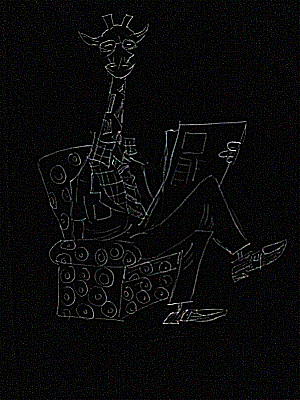
\includegraphics[width=2in]{org/art/takingHelp.png}\end{center}
\end{wrapfigure}

%Are you demotivated? Do you find the world uninspirational. Do you find yourself yourself left out in the world without keeping pace with rapidly progressing technology. You may probably find peace in development. Development is awesome because it gives you the feeling of God. You create and see your things working.
%\linebreak
%\par
%As a developer, its your religion to try every stuff out there. This book is about taking shortcuts to get your 'thing' running. This book targets only a specific set of technology. You may choose to differ and take a different path.
%\linebreak
%\par
%Hopefully, it will give you a drift and get started. You will have to solve your itches and tackle issues yourself. However, 

I will follow a particular set of technology to demonstrate how to build a web application for your needs. The demo app will be a movie site, much like IMDB, just that it would be more user centric.

When you are stuck Stackoverflow will be your best friend. Most of your queries will be already answered there. Next best friend is Google. And when you feel like expert of nodejs and can't find answers online, you can even join the mailing list.

%You could opt for asking questions at the nodejs mailing list, but subscribing will mean lot of emails every day as node is quite a hot topic these days.
%Also, it might be demotivational because you will see people building fantastic things and their progress is much faster than yours.
%So, initially you might want to focus on fixing your problems before you catch speed.
%the survival tale/keeping alive - airbnb for motivation

%\begin{flushright}\textit{Its better to burn out than to fade away.}\end{flushright}
%What is this book about? This book is intended to serve as a tutorial to build your applications quickly.


\chapter{Quick Launch}
\begin{flushright}\textit{It seems I am on speed.}\end{flushright}

\begin{wrapfigure}{r}{2in}
\begin{center}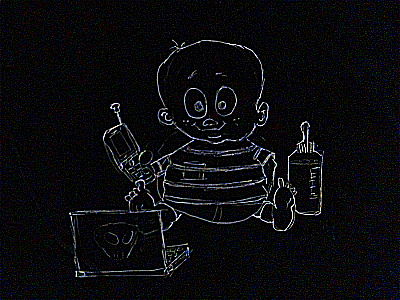
\includegraphics[width=2in]{org/art/getStartedHigh.png}\end{center}
\end{wrapfigure}

Nothing gives a better kick than working and releasing fast. The following code will get you a ``launching soon'' page ready with beta invite albeit manually. It requires node.js, an evented IO framework by Ryan Dahl. The code itself is written in coffeescript, a language by Jeremy Ashkenas.
First be comfortable with code and the fact that this small code will get us started and then we can move on to get it working.

\vspace{0.6cm}\lstinputlisting{app/stage1/server.coffee}\vspace{0.6cm}

%tip
\colorbox{tipcolour}{\tiny \textsc{Tip} \small Use commercial solutions like unbounce to set up quick sign up page}


%\chapter{Working Model}
%\begin{flushright}\textit{If it doesn't work, it doesn't exist.}\end{flushright}

%\begin{wrapfigure}{r}{2in}
%\begin{center}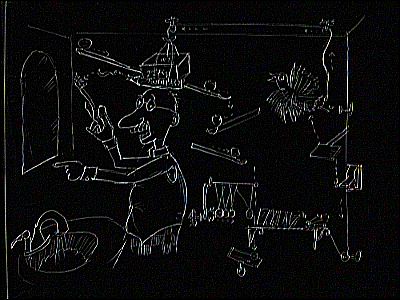
\includegraphics[width=2in]{org/art/workingModel.png}\end{center}
%\end{wrapfigure}

%Last stage was a baby's task. Lets get real and get a working model. To keep it simple, lets stick with simplest authentication via facebook and build upon existing hardwork. MongoDB will be used for storage, though a document based database is not really an ideal choice for the purpose. 


\chapter{Express}
\begin{flushright}\textit{Run. Run. Run.}\end{flushright}

\begin{wrapfigure}{r}{2in}
\begin{center}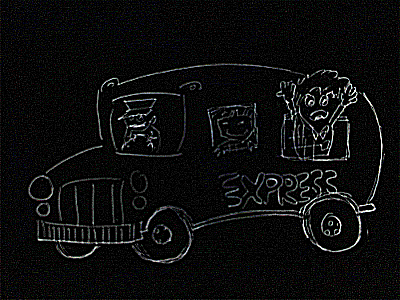
\includegraphics[width=2in]{org/art/fasterEasier.png}\end{center}
\end{wrapfigure}

Time to take the express. A quick reorganization of code so as to switch to a big framework which will make life easier in long run. As you can figure out we don't need to parse req.url and add switch statement to handle different url, if we stuck to last example. Express makes routing a breeze.

\vspace{0.6cm}\lstinputlisting{app/stage2/server.coffee}\vspace{0.6cm}



\chapter{Database}
\begin{flushright}\textit{You can has data.}\end{flushright}

\begin{wrapfigure}{r}{2in}
\begin{center}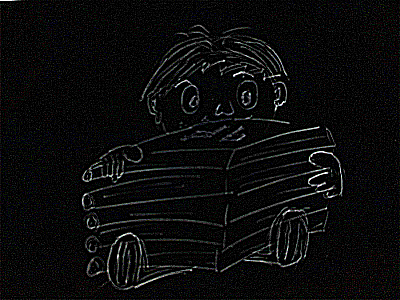
\includegraphics[width=2in]{org/art/dataStorage.png}\end{center}
\end{wrapfigure}

MongoDB will store our data. Note that we have to think asynchronously. The database choice here was dictated more by ease rather than a good fit. In fact, a document based database in not really optimal for storing relational data.
Lets focus on the working example which pulls the data from the database. Visit mongodb website for installation, building a database and storing dummy data. We will use mongoose module to interact with the server.

\vspace{0.6cm}\lstinputlisting{app/stage3/server.coffee}\vspace{0.6cm}

%tip
%\noindent
Movie data can be inserted via mongo command line interface \\
\colorbox{tipcolour}{\tiny \textsc{Tip} \small ./mongodb-linux-i686-1.6.5/bin/mongod --dbpath ./data/db/ } \\
\colorbox{tipcolour}{\tiny \textsc{Tip} \small ./mongodb-linux-i686-1.6.5/bin/mongo localhost/db } \\
\par

%or via node application
%\begin{lstlisting}
%mongoose = require 'mongoose';
%mongoose.connect 'mongodb://localhost/db';
%require './models/movie';
%movie = mongoose.model 'movie';
%d = new movie();
%d.id = 2;
%d.name = 'Andaz Apna Apna';
%d.save (err) ->
%	if (err)
%		console.log 'error: ' + e;
%	mongoose.disconnect();
%\end{lstlisting}




\chapter{Intermission}
\begin{flushright}\textit{Organize your data before you die.}\end{flushright}

\begin{wrapfigure}{r}{2in}
\begin{center}
\includegraphics[width=2in]{org/art/organized.png}\end{center}
\end{wrapfigure}

We will stick to a common layout in order to keep the code organized in long run. It also makes it easier to understand and maintain. Here, models directory will contain the data models corresponding to the database. Controllers will be handlers of different type of requests. The views will contain Jade templates which will be rendered by the jade module.
\linebreak

\begin{verbatim}
       app.coffee               (our application)
       |--models                (contains data models)
       |--views                 (jade templates)
       |--controllers           (handler for different requests)
       |--data                  (data storage)
          |--db
       |--public                (static content)
          |--js
          |--css
          |--img
\end{verbatim}

\par
\vspace{1cm}

According to this scheme, the contents will now be\\
\lstinputlisting[title={app.coffee}]{app/stage4/app.coffee}\vspace{0.6cm}
\lstinputlisting[title={movie controller}]{app/stage4/models/movie.coffee}\vspace{0.6cm}
\lstinputlisting[title={homepage controller}]{app/stage4/controllers/home.coffee}\vspace{0.6cm}
\lstinputlisting[title={movie model}]{app/stage4/controllers/movie.coffee}\vspace{0.6cm}

Current example doesn't really use templates because we are just refactoring the code from last chapter. But the organisation reflects how we want to categorize similar type of source files in the same organisation hierarchy under same directory.


%Dealing with image data
%We can store it at EC2 and refer to its location in the database


% references tpwbooks, dhh

\end{document}
